\section{Snapshotting memory-based state machines}
\label{compaction:memsnapshot}

The first approach to snapshotting applies when the state machine's data
structures are kept in memory. This is a reasonable choice for state
machines with datasets in the gigabytes or tens of gigabytes. It
enables operations to complete quickly, since they never have to fetch
data from disk; it is also easy to program, since rich data
structures can be used and every operation can run to completion
(without blocking for I/O).

\begin{figure}
\centering
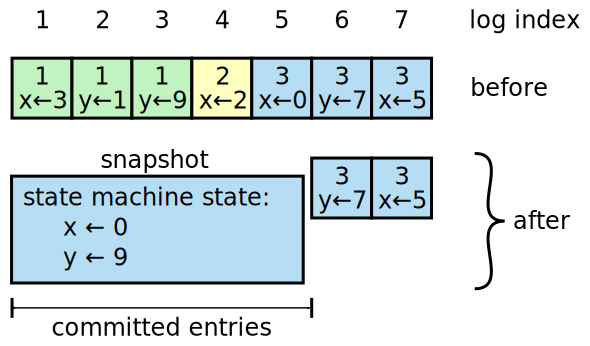
\includegraphics[scale=.50]{compaction/snapshot}
\vcaption[memory-based snapshotting approach]{
A server replaces the committed entries in its log (indexes 1 through 5)
with a new snapshot, which stores just the current state (variables
$x$ and $y$ in this example). Before discarding entries 1 though 5,
Raft saves the snapshot's last included
index (5) and term (3) to position the snapshot in the log preceding
entry 6.
}
\label{fig:compaction:snapshot}
\end{figure}

Figure~\ref{fig:compaction:snapshot} shows the basic idea of
snapshotting in Raft when the state machine is kept in memory. Each
server takes snapshots independently, covering just the committed
entries in its log. Most of the work in snapshotting involves
serializing the state machine's current state, and this is specific to a
particular state machine implementation. For example, LogCabin's
state machine uses a tree as its primary data structure; it serializes
this tree using a pre-order depth-first traversal (so that when
applying the snapshot, parent nodes are created before their children).
State machines must also serialize the information they keep for
providing linearizability to clients (see Chapter~\ref{clients}).

Once the state machine completes writing a snapshot, the log can be
truncated. Raft first stores the state it needs for a restart:
the index and term of the last entry included in the snapshot and the
latest configuration as of that index. Then it discards the prefix of
its log up through that index. Any previous snapshots can also be
discarded, as they are no longer useful.

\begin{figure}
\centering
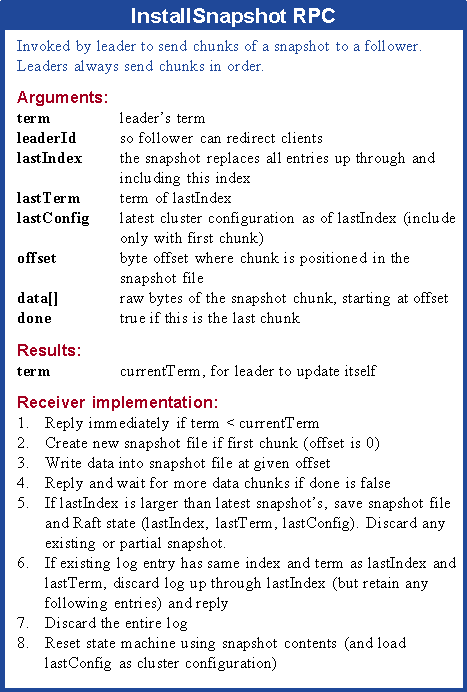
\includegraphics[scale=1.0]{compaction/cheatsheet}
\vcaption[InstallSnapshot RPC]{
Leaders invoke the InstallSnapshot RPC to send snapshots to slow
followers. Leaders resort to sending a snapshot only when they
have already discarded the next log entry needed to
replicate entries to the follower with AppendEntries.
They split the snapshot into chunks for transmission. Among other
benefits, this gives the follower a sign of life with each chunk, so it
can reset its election timer. Each chunk is sent in order, which
simplifies writing the file to disk.
The RPC includes the state needed for Raft to load the snapshot on a
restart: the index and term of the last entry covered by the snapshot,
and the latest configuration at that point.
}
\label{fig:compaction:cheatsheet}
\end{figure}

As introduced above, the leader may occasionally need to send its state
to slow followers and to new servers that are joining the cluster. In
snapshotting, this state is just the latest snapshot, which the leader
transfers using a new RPC called InstallSnapshot, as shown in
Figure~\ref{fig:compaction:cheatsheet}.
When a follower receives a snapshot with this RPC, it must decide
what to do with its existing log entries.
Usually the snapshot will
contain new information not already in the follower's log.
In this case, the follower discards its entire log; it is all
superseded by the snapshot and may possibly have uncommitted entries
that conflict with the snapshot. If, instead, the follower receives a
snapshot that describes a prefix of its log (due to retransmission or by
mistake), then log entries covered by the snapshot are deleted but
entries following the snapshot are still valid and must be retained.

The remainder of this section discusses secondary issues for
snapshotting memory-based state machines:
%
\begin{compactitem}
%
\item Section~\ref{compaction:memsnapshot:concurrent} discusses how to
produce snapshots in parallel with normal operations, to minimize their
effects on clients;
%
\item Section~\ref{compaction:memsnapshot:when} discusses when to take a
snapshot, balancing the space usage and the overhead of snapshotting; and
%
\item Section~\ref{compaction:memsnapshot:implementation} discusses the
issues that arise in implementing snapshotting.
%
\end{compactitem}

\subsection{Snapshotting concurrently}
\label{compaction:memsnapshot:concurrent}

Creating a snapshot can take a long time, both in serializing
the state and in writing it to disk. For example, copying
\SI{10}{\giga\byte} of
memory takes about one second on today's servers, and serializing it
will usually take much longer: even a solid state disk
can only write about \SI{500}{\mega\byte} in one second.
Thus, both serializing and
writing snapshots must be concurrent with normal operations to avoid
availability gaps.

Fortunately, copy-on-write techniques allow new updates to be applied
without impacting the snapshot being written.
There are two approaches to this:
%
\begin{itemize}
%
\item State machines can be built with immutable (functional) data
structures to support this. Because state machine commands would not modify
the state in place, a snapshotting task could keep a reference to
some prior state and write it consistently into a snapshot.
\item
Alternatively, the operating system's copy-on-write support can be used
(where the programming environment allows it).
On Linux for example, in-memory state machines can use \emph{fork} to make a
copy of the server's entire address space. Then, the child process can
write out the state machine's state and exit, all while the parent
process continues servicing requests. The LogCabin implementation
currently uses this approach.
\end{itemize}

Servers require additional memory for snapshotting concurrently, which should be
planned for and managed. It is essential for state machines to have a
streaming interface to the snapshot file, so that the snapshot does not
have to be staged entirely in memory while it is created. Still,
copy-on-write requires extra memory proportional to the fraction of the
state machine state that is changed during the snapshotting process. Moreover, relying on
the operating system for copy-on-write will typically use even more
memory due to false sharing (for example, if two unrelated data items
happen to be on the same page of memory, the second item will be
duplicated even when only the first has changed). In the unfortunate
event that memory capacity is exhausted during snapshotting, a server should
stop accepting new log entries until it completes its snapshot; this
would temporarily sacrifice the server's availability (the cluster might
still remain available), but at least it would allow the server to
recover. It is better not to abort the snapshot and retry later,
since the next attempts might also face the same problem.
(LogCabin uses a streaming interface to disk, but it does not currently
handle memory exhaustion gracefully.)


\subsection{When to snapshot}
\label{compaction:memsnapshot:when}

Servers must decide when to snapshot. If a server snapshots too often,
it wastes disk bandwidth and other resources; if it snapshots too
infrequently, it risks exhausting its storage capacity, and it increases
the time required to replay the log during restarts.

One simple strategy is to take a snapshot when the log reaches a fixed
size in bytes. If this size is set to be significantly larger than the
expected size of a snapshot, then the disk bandwidth overhead for
snapshotting will be small. However, this can result in needlessly large
logs for small state machines.

A better approach involves comparing the snapshot's size with the log's
size. If the snapshot will be many times smaller than the log, it is
probably worthwhile to take a snapshot. However, calculating the size of
a snapshot before it is taken can be difficult and burdensome, imposing
a significant bookkeeping burden for the state machine, or requiring
almost as much work as actually taking a snapshot to compute the size
dynamically. Compressing snapshot files also results in space and
bandwidth savings, but it is hard to predict how large the compressed
output will be.

Fortunately, using the size of the \emph{previous} snapshot rather than
the size of the next one results in reasonable behavior. Servers take a
snapshot once the size of the log
exceeds the size of the previous snapshot times a configurable
\emph{expansion factor}. The expansion factor trades off disk bandwidth
for space utilization. For example, an expansion factor of 4 results in
about 20\% of the disk's bandwidth being used towards snapshotting (for
every 1 byte of snapshot, 4 bytes of log entries will be written), and
requires about 6 times the disk capacity as that needed to store a
single copy of the state (the old snapshot, a log 4 times bigger than
that, and the new snapshot being written).

Snapshotting still creates a burst of CPU and disk bandwidth usage that
might impact client performance. This can be mitigated with additional
hardware; for example, a second disk drive can be used to provide the
additional disk bandwidth.

It may also be possible to schedule snapshots in a way that client
requests never wait on a server that is snapshotting. In this approach,
servers would coordinate so that only up to a minority of the servers in
the cluster would snapshot at any one time (when possible). Because Raft
only requires a majority of servers to commit log entries, the minority of
snapshotting servers would normally have no adverse effect on clients.
When a leader wished to snapshot, it would step down first,
allowing another server to manage the cluster in the meantime. If this
approach was sufficiently reliable, it could also eliminate the need to
snapshot concurrently; servers could just be unavailable while they took
their snapshots (though they would count against the cluster's
ability to mask failures). This is an exciting opportunity for future
work because of its potential to both improve overall system performance
and reduce mechanism. 

%


\subsection{Implementation concerns}
\label{compaction:memsnapshot:implementation}

This section reviews the major components needed for a snapshotting
implementation and discusses the difficulties with implementing them:
%
\begin{itemize}
%
\item \textbf{Saving and loading snapshots:}
%
Saving a snapshot involves serializing the state machine's state and
writing that data out to a file, while loading is the reverse process.
We found this to be fairly straightforward, although it was somewhat
tedious to serialize the various types of data objects from their native
representations. A streaming interface from the state machine to a file
on disk is useful to avoid buffering the entire state machine state in
memory; it may also be beneficial to compress the stream and apply a
checksum to it.
LogCabin writes each snapshot to a temporary file first, then renames
the file when writing is complete and has been flushed to disk; this
ensures that no server loads a partially written snapshot on startup.

%
\item \textbf{Transferring snapshots:}
%
Transferring snapshots involves implementing the leader and follower
sides of the InstallSnapshot RPC. This is fairly straightforward and may
be able to share some code with saving snapshots to and loading
snapshots from disk.
The performance of this transfer is usually not very important (a
follower that needs this state has not been participating in the
commitment of entries, so it is probably not needed soon; on the other
hand, if the cluster suffers additional failures,
it may need to catch up the follower to restore availability).
%
\item \textbf{Eliminating unsafe log accesses and discarding log
entries:}
%
We originally designed LogCabin without worrying about
log compaction, so the code assumed that if entry $i$ was present in the
log, entries $1$ through $i - 1$ would also be present. This is no
longer true with log compaction; for example, when determining the term
for the previous entry in the AppendEntries RPC, that entry might have
been discarded.
Removing these assumptions throughout the code required careful
reasoning and testing. This would have been easier with help from a more
powerful type system, if the compiler could enforce that every access to
the log also handled the case that the index was out of bounds.
Once we had made all the log accesses safe, discarding the prefix of
the log was straightforward. Until this point, we could only test the
saving, loading, and transferring snapshots in isolation, but when log entries can be safely
discarded, these can all start to be exercised in
system-wide tests.
%
\item \textbf{Snapshotting concurrently with copy-on-write:}
%
Snapshotting concurrently may require reworking the state machine or
leveraging the operating system's fork operation. LogCabin currently
uses fork, which interacts poorly with threads and C++
destructors; getting this to work correctly presented some
difficulty. However, it is a small amount of code and completely
eliminates the need to modify the state machine's data structures, so we
think it was the right approach.
%
\item \textbf{Deciding when to snapshot:}
%
We recommend taking snapshots after applying every log entry during
development, since that can help catch bugs quickly. Once the
implementation is complete, a more useful policy of when to snapshot
should be added (e.g., using statistics about the size of Raft log and the
size of the last snapshot).
%
\end{itemize}

We found piecewise development and testing of snapshotting to be
challenging. Most of these components must be in place before it is
possible to discard log entries, but only then will many of the new code
paths be exercised in system-wide tests. Thus, implementers should
consider the order in which to implement and test these components carefully.
